\documentclass[11pt]{article}
% \setlength{\parindent}{0pt}
% \setlength{\parskip}{10pt}

\usepackage{arxiv}

\usepackage{graphicx}
\usepackage{indentfirst,csquotes}
\usepackage{amssymb,amsthm,amsmath}
\usepackage{hyperref}
\usepackage{cite}
\usepackage{enumitem}
\usepackage{lmodern}
\usepackage{fancyhdr}

% rewrite font for compiling warning
\usepackage{times}
% rewrite page head
\rhead{}

% \topmargin= .5cm
% \textheight= 20cm
% \textwidth= 32cc
% \baselineskip=16pt
% \evensidemargin= .9cm
% \oddsidemargin= .9cm


% \pagestyle{fancy}
% \fancyhf{}
% \fancyfoot[C]{\thepage}
% \renewcommand{\headrulewidth}{0pt}


\hypersetup{
  colorlinks=true,
  linkcolor=blue,
  citecolor=black,
  urlcolor=blue
}


\begin{document}

\title{
Sentiment of movie review analysis by Random forest, LSTM and Bert
}

\author{
  Xinfang Li(1591669), Xueyan Hu(1586157), Jia Zhang (1578438)
}
\date{\today}

\maketitle
\markboth{}{}

\begin{abstract}
% importance and challenge
% introduce ML and DL
% introduce datasets
% summary the results
Sentiment analysis plays a critical role for figuring out the meaningful information from movie reviews. Its ability is to process vast amounts of data collected from social media, review websites and personal blogs and get the emotional tendency behind the words, then, the process transforms the opinions into quantifiable data offering insights of audience preferences and the trends of the market. The analysis results are valuable for filmmakers and distributors of movie to adapt their strategies to attract more audience. However, the challenges significantly impact the tasks implementation, such as processing huge data collections. This project introduces two kind of computing powered methods, machine learning (ML) including Random Forest and Long Short Term Memory (LSTM), deep learning (DL) like Bidirectional Encoder Representations from Transformers (BERT), to handle this challenge. The Standford IMDb dataset from HuggingFace was used for training and to evaluate the performance by accuracy, classification report and confusion matrix. The models achieves the accuracy by 85.4\%, 85.5\% and 94.0\% respectively for sentiment classification.
\end{abstract}

\clearpage
\thispagestyle{empty}
\tableofcontents
\thispagestyle{empty}

\clearpage
\setcounter{page}{1}

% introduction
% Domain, Problem, Literature review, Solution, methodology and What this report does
\section{Introduction}

\subsection{Domain and problem}
In this project, the key domain is natural language processing (NLP), which focuses on extracting information, such as emotions or opinions, from the given content. The reviews of movie classification is a classic problem where sentiment, including positive and negative, is predicted based on the context of reviews, its applications are verity including renewcommand systems and business intelligence. The primary challenge is to capture the nuances and semantic relationships in the content accurately particularly when dealing with the complex language. 

\subsection{Literature review}
A research \cite{pang2008opinion} introduces machine learning (ML) techniques to classify the review depend on its sentiment, which achieves high accuracy in prediction of audience opinions. It is a practical application for this kind of project to understanding the viewers' preferences and improve the film industry's decision making. 

Pang et al. (2022) pioneered using ML for movie review sentiment classification \cite{pang2002thumbs}, and more recent works demonstrate that ensemble methods like Random Forests, outperform simpler models such as Naive Bayes, or Logistic Regression in many real-world settings \cite{breiman2001random,go2009twitter}. Moreover, datasets like the Standford IMDB dataset \cite{maas2011learning} have become benchmarks for evaluating models. Random Forest is chosen as one candidate, because it can work robustly and efficiently when handling high-dimensional textual content in classification tasks \cite{kowsari2019text}. 

Long-Short-Term Memory (LSTM) has also shown a significant advantages in textual content sentiment analysis. For instance, Johnson and Zhang (2016) introduced an efficiently LSTM framework which is using a general "region embedding plus pooling" paradigm \cite{johnson2016supervised}. They feed one-hot vectors into LSTM units instead of the word embedding layer. In this architecture, they built a one-hot bidirectional LSTM with pooling (oh-2LSTMp), which achieved a test error rate by 8.14\%, and in the supervised setting by 6.66\%. Sachan et al. (2019) developed a bidirectional LSTM model, which trained with supervised and semi-supervised losses, the model achieved 4.32\% error rate on IMDB dataset \cite{sachan2019revisiting}.

Deep learning (DL) has revolutionized ability to solve NLP problems by enabling models to learn complex patterns from large datasets. It surpasses traditional ML approaches in the sentiment analysis tasks. The deep learning models, for example, RNNs (recurrent neural networks) and CNNs (convolutional neural networks), extract features from the content automatically. However, these models often struggling with capturing long dependencies, which limits its performance in the tasks. 

Devlin et al. (2018) introduce BERT, Bidirectional Encoder Representations from Transformers, for handling the classification tasks with significant advancement. BERT leverages a bidirectional transformer architecture, which allows it to capture the context from preceding and following words. It combines with pre-trained on vast corpora and next-sentence prediction, which enables BERT to generate rich representations \cite{Devlin2018}. In sentiment analysis, BERT excels by modeling complex relationships between words in textual content. For example, Sun et al. (2019) demonstrated BERT's advantage in sentiment analysis, it outperforms RNNs and CNNs, and achieves robust performance with limited labeled data \cite{Sun2019}. However, this methods also cause challenges such as computational complexity and resource demands.

\subsection{Dateset}
The IMDB dataset is used commonly to evaluate sentiment classification tasks. It exactly includes 50 thousand reviews of movies, and it is split into 25,000 positive and same number of negative reviews equally, which means that it is a balanced dataset. This feature ensures no class imbalance issues which influences the accuracy of the results. Every sample is labeled as either positive by 1 or negative by 0, which means it is a binary-classifying task. This dataset is originally divided into training (50\%) and testing (50\%) sets. All selected methods are trained and evaluated on this dataset.

\begin{figure}[ht]
    \centering
    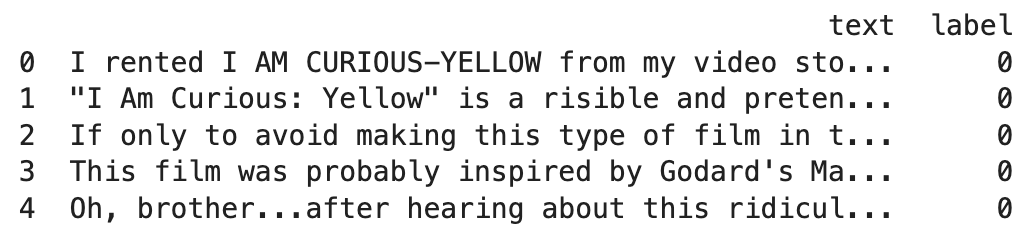
\includegraphics[width=0.6\textwidth]{pics/data_sample.png}
    \caption{Dataset samples}
\end{figure}

\subsection{Solution}
To address the sentiment classification task based on IMDb training and evaluation dataset \cite{stanfordnlp2025imdb}, we propose three distinct machine learning models: Random Forest, LSTM networks and BERT. These models are selected to capture the dependencies between words in long sequence, the models include traditional methods and deep learning techniques. This strategy allows us to compare their effectiveness in this textual classification. Random Forest leverages tree-based learning, LSTM captures sequential dependencies in content, and BERT utilizes contextual embeddings to understand semantic representations. After evaluation, our goal is to figure out the best method of them for sentiment classification on the selected dataset.

The methodology for this project includes the following steps:
\begin{enumerate}
    \item Data preparation
    \item Model implementation
    \item Training and Evaluation
    \item Comparison and Analysis
\end{enumerate}


\subsection{What this report does}
This report compares Random Forest, LSTM, and BERT in the sentiment classifying task. It details the implementation, training and evaluating for each model, then it provides insights into their strengths and weaknesses. It also demonstrates the processing steps, feature engineering techniques and fine tuning method. To compare and analyzing the results, the recommendations on the most suitable model are identified for sentiment classification, which contributes how traditional and deep learning approaches perform on textual content.

% methods
\section{Methodology of Random Forest}

The sentiment analysis base on RF pipeline can be visually and logically described with the following flowchart:

\begin{figure}[ht]
    \centering
    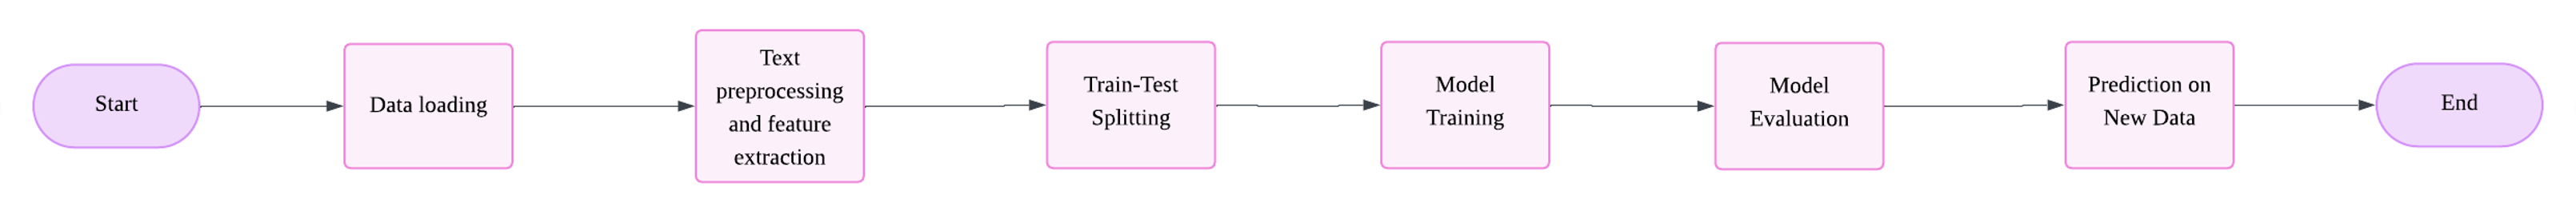
\includegraphics[width=1\textwidth]{pics/rf_steps.png}
    \caption{Random Forest analysis pipeline}
\end{figure}

\subsection{Step-by-step inputs and outputs}

\subsubsection*{Dataset Loading}
The first step is acquiring the dataset. We use the IMDB movie review dataset which is available on HuggingFace under the ID "stanfordnlp/imdb". The data is loaded using the "load\_dataset" function from HuggingFace's datasets library. After loading, it is converted into a pandas DataFrame to facilitate further processing.

Input: Dataset is fetched automatically.\\
Process: Dataset is downloaded and parsed.\\
Output: A structured dataset with two columns: text (the review) and label (the sentiment class).

\subsubsection*{Text Preprocessing and Feature Extraction}
Machine learning models cannot interpret raw textual data directly. Therefore, we must convert each review into a numerical representation. This is done using TF-IDF (Term Frequency-Inverse Document Frequency) vectorization.

TF-IDF calculates the importance of a word in a document relative to all other documents. We use the Tf-IDF Vectorizer from scikit-learn configured with "max\_features" as 10000 to limit vocabulary size and stop\_words as 'english' to remove commonly used words that carry little sentiment meaning.
This process transforms the review texts into a high-dimensional sparse matrix, where each row represents a review and each column represents a word feature.

Input: Raw review texts and labels.\\
Process: Tokenization, stopword removal and TF-IDF computation.\\
Output: A TF-IDF feature matrix X\_vec with shape.

\subsubsection*{Train-Test Splitting}
In this step, we split the dataset into training and testing subsets using scikit-learn's "train\_test\_split" function. We allocate 80\% of the data to training and 20\% to testing. The split is randomized but reproducible due to a fixed random seed by setting "random\_state" as 42.
This step ensures that the model is trained on one portion of the data and evaluated on completely unseen data, which simulates a real-world deployment scenario.

Input: TF-IDF feature matrix X\_vec and label vector y. \\
Process: Random partitioning of data into training and test sets. \\
Output: X\_train and y\_train used to train the model, X\_test and y\_test used to evaluate the model.

\subsubsection*{Model Training}
We train a Random Forest Classifier which is an ensemble learning algorithm. It creates multiple decision trees and combines their predictions to improve accuracy and reduce overfitting.
The classifier is instantiated using scikit-learn's RandomForestClassifier. For the initial experiment, we use default settings with "n\_estimators" as 100, which means 100 decision trees are built.
The training data (X\_train and y\_train) is fed into the "fit" function, which constructs the trees by learning patterns in the TF-IDF features that differentiate positive and negative reviews.

Input: X\_train (TF-IDF vectors) and y\_train (labels). \\
Process: Each tree learns decision rules from data subsets and the forest aggregates these decisions.\\
Output: A trained RandomForestClassifier model object.

\subsubsection*{Model Evaluation}
After training, we evaluate the model's ability to classify reviews it has never seen before. This is done using the test set (X\_test, y\_test).
We use the "predict" method to generate predicted labels and then calculate performance metrics. These metrics help understand both overall accuracy and error distribution which is especially important in binary classification tasks.

\begin{itemize}
    \item Accuracy: the proportion of correct predictions
    \item Classification Report: includes precision, recall and F1-score
    \item Confusion Matrix: shows how many true/false positives and negatives the model predicted
\end{itemize}

Input: Trained model, X\_test and y\_test. \\
Process: Predict labels and compare against true values \\
Output: Accuracy score, detailed classification report and confusion matrix.

\subsubsection*{Prediction on New Data}
Finally, the trained model can be used to predict sentiment on new movie reviews provided by users. Before prediction, the new review text must go through the same TF-IDF transformation as the training data.
The "vectorizer.transform" method is used to convert raw text to a vector which is then passed to the model's "predict" method.

Input: New review text. \\
Process: Apply TF-IDF vectorization, ten make prediction. \\
Output: A sentiment prediction 0 (negative) or 1 (positive).


\subsection{Implementation of Random forest}
The implementation of this sentiment analysis project is fully contained, which consists of the following key components.

\begin{enumerate}
    \item Loading the IMDB Dataset from HuggingFace: The script uses the datasets library to automatically fetch the standfordnlp/imdb dataset. Only the labeled train and test splits are used. The data is then converted into pandas DataFrames for ease of manipulation and preprocessing.
    \item TF-IDF Vectorization: The text data is transformed into numerical features using TF-IDF Vectorizer from scikit-learn. The vectorizer is configured with max\_features as 10000 and stop\_words as 'english' to ensure a compact, meaningful vocabulary. This transforms raw text into a sparse matrix of features suitable for machine learning.
    \item Model Training and Prediction Using Random Forest: A RandomForestClassifier is initialized with 100 decision trees. The classifier is trained on the training set and then tested to obtain the sentiment predictions on the test data.
    \item Evaluation Metrics Output: After prediction, the script computes accuracy score, confusion matrix, classification report including precision, recall and F1-score. These metrics provide a comprehensive view of how well the model performs on unseen data.
    \item Confusion Matrix Visualization and Saving: The confusion matrix is plotted as a heatmap for better readability and visual analysis. The resulting plot is saved as an image file.
\end{enumerate}


\subsection{Results of random forest}
In this section, we present the experimental results obtained from training and evaluating the Random Forest classifier on the IMDB movie review dataset. The results are discussed in terms of standard classification metrics including accuracy, precision, recall, F1-score and confusion matrix.
After training the model on the preprocessed TF-IDF features and evaluating it on the unseen test set, the model achieved accuracy: 85.3\%. This shows that the Random Forest model is able to correctly classify the sentiment of about 8.5 out of every 10 reviews. Given the simplicity of the feature representation, this is a strong baseline.

\subsubsection*{Classification Report}
\begin{figure}[ht]
    \centering
    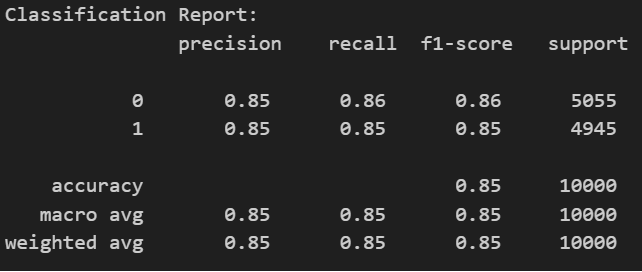
\includegraphics[width=0.5\textwidth]{pics/rf_eval_report.png}
    \caption{Classification Report of Random Forest}
\end{figure}

Precision: When the model predicts a sentiment, it is correct about 85\% of the time.
Recall: The model is slightly lower at identifying positive reviews than negative ones.
F1-score: A good balance between precision and recall, indicating consistent performance.

\subsubsection*{Confusion Matrix}
This confusion matrix shows the number of true/false predictions made by the classifier:

\begin{figure}[ht]
    \centering
    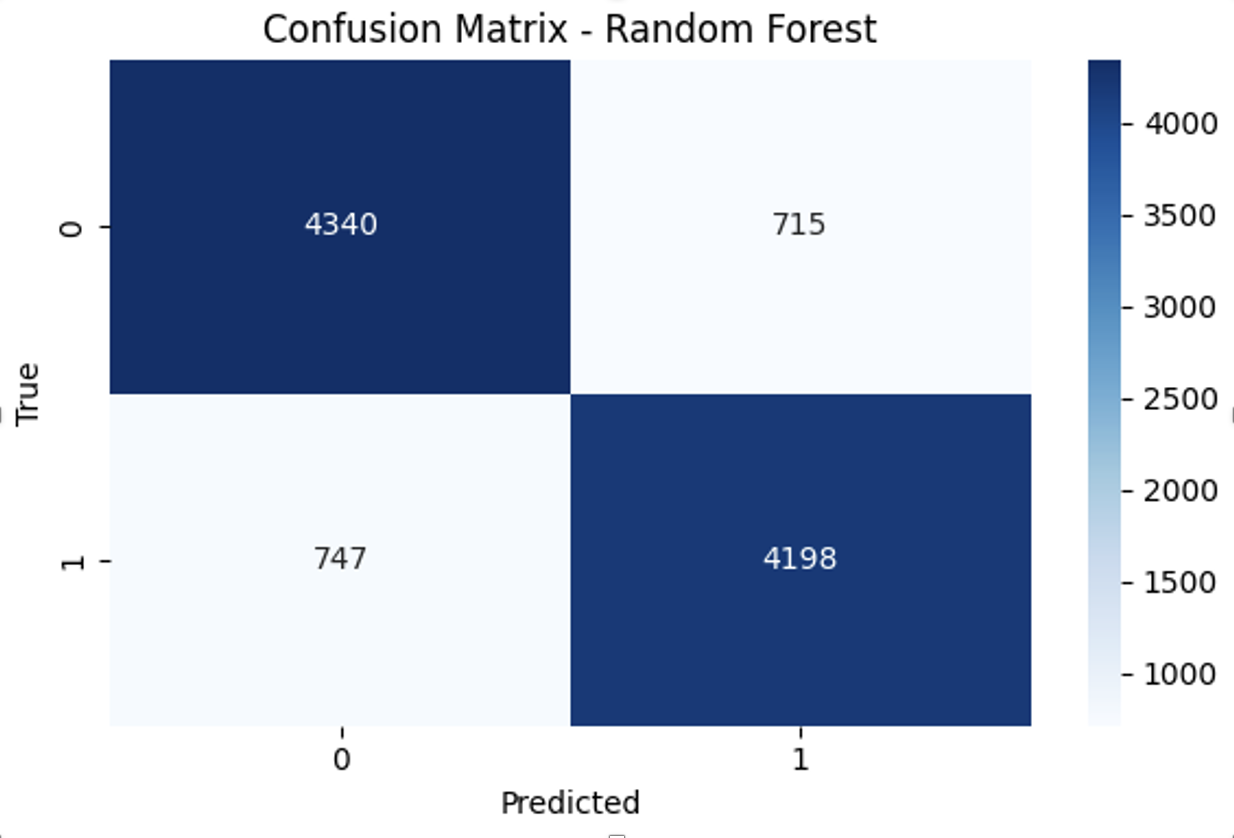
\includegraphics[width=0.4\textwidth]{pics/rf_eval_metrix.png}
    \caption{Confusion Matrix of Random Forest}
\end{figure}

Interpretation:
True Negatives (TN): 4340 —— correctly predicted negative reviews.
False Positives (FP): 715 —— negative reviews incorrectly predicted as positive.
False Negatives (FN): 747 —— positive reviews incorrectly predicted as negative.
True Positives (TP): 4198 —— correctly predicted positive reviews.

\subsubsection*{Conclusion}
Random Forest proves to be a reliable and interpretable model for sentiment analysis of movie reviews. While deep learning methods may offer marginal gains, ensemble methods like Random Forest offer a good balance between performance and computational efficiency.



\section{Methodology of LSTM}
LSTM is a special Recurrent Neural Network(RNN) \cite{sak2014long}. It is able to learn from sequential data quickly, during this process, it captures long-and-short term dependencies in the sequence. Because LSTM involves the memory cell, which is including input, forget and output gate.

\begin{figure}[ht]
    \centering
    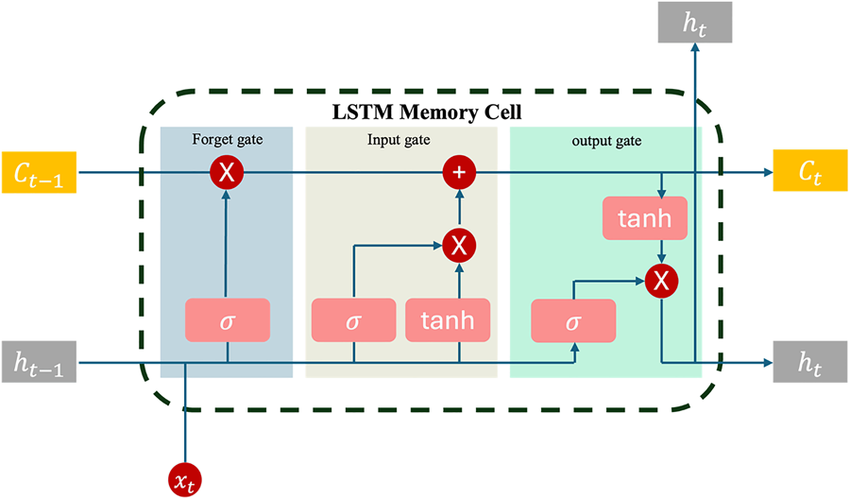
\includegraphics[width=0.7\textwidth]{pics/lstm_memory_cell.png}
    \caption{The architecture of memory cell in LSTM (Source: Dual-transformer deep learning framework \cite{chen2025dual})}
\end{figure}

LSTM can gain or drop information depend on it selection when a state of cell through these gates. This mechanism makes the model performing well in natural language text. It can automatically learn features from raw sequences so that we don't need to construct features like n-gram and TF-IDF. Furthermore, compared to standard Recurrent Neural Networks, LSTMs are specifically designed to address the diminishing gradient issues, which allows them to remember information across longer text spans, a crucial advantage for sentiment analysis tasks.

\subsection{Model Architecture design}
We built the LSTM model with the following steps: processed raw IMDb data into padded integer sequences, added embedding and LSTM layer to extract features, then regularized with dropout, and finally get sentiment classification through a sigmoid activated dense layer.

\begin{figure}[ht]
    \centering
    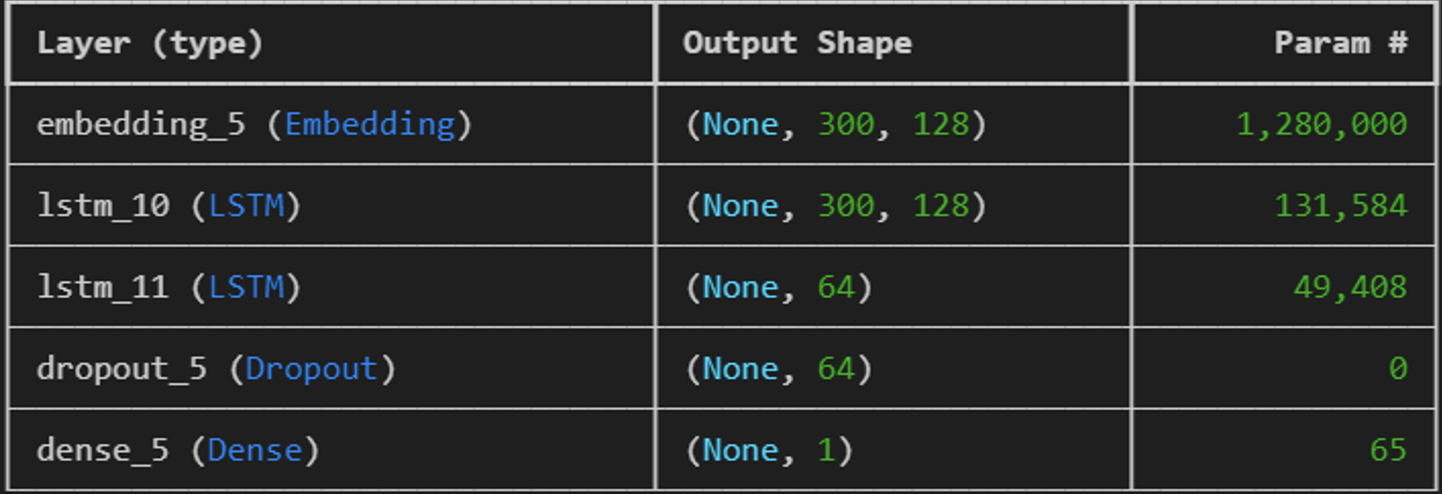
\includegraphics[width=0.6\textwidth]{pics/lstm_model.png}
    \caption{The model review of LSTM}
\end{figure}

The pipeline began with raw IMDb reviews. We proprocessed the data by mapping each word into an integer index and then padding all sequences to a length of 300 tokens. This allowed the data to be trained efficiently in batches. Next we built an Embedding layer, which serves as the input layer. It transforms the integer-encoded vocabulary (limited to the 10,000 most frequent words) into dense, 128-dimensional vectors. This layer is crucial as it learns a meaningful, continuous representation for each word that captures semantic relationships within the vector space.

Next, we stack two LSTM layers to model temporal dependencies in the text. The first LSTM includes 128 hidden units, and it outputs the entire hidden states as a sequence. This seconde LSTM layer has 64 hidden units and outputs only a hidden state from the final time step. This single vector acts as a powerful summary of the entire input sequence, encoding the sentiment of the review.

To reduce the risk of overfitting, dropout layers are added between the LSTM stacks, the drop rate is setting as 0.4, the final dense output layer also added for the same reason. The last layer used a single neuron activated by sigmoid function to predict the probability of the review being positive. The training was performed by using the "Adam" optimization algorithm and Binary cross-entropy (BCE) loss, with model performance evaluated through both accuracy and AUC metrics.

\subsection{Results of LSTM}
After training 50 epochs of our LSTM model, we evaluated it on an unseen test set. Our model got 85.5\% accuracy in the test set, and 88\% of Area Under the ROC Curve (AUC). The results illustrates that our LSTM model has successfully learned sentiment-relevant features from the data.

The classification report showed almost similar value of precision, recall, and F1-scores in positive-negative classes. They all approached around 0.855 which indicates that the model treated both positive and negative reviews with equal effectiveness and no bias.

\begin{figure}[ht]
    \centering
    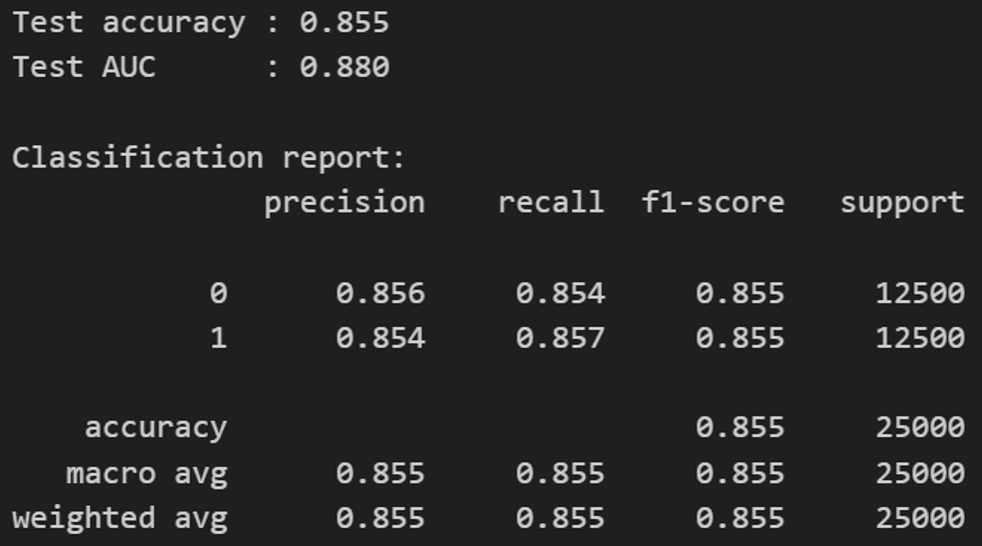
\includegraphics[width=0.5\textwidth]{pics/lstm_report.png}
    \caption{The classification report of LSTM}
\end{figure}

In the confusion matrix, the diagonal values (TN, TP) are much higher than off-diagonal (FP, FN) which shows a high correct rate prediction along the main diagonal versus incorrect predictions. The counts of failed prediction in positives and negatives are very similar, 1827 and 1791 respectively. This balance also supported that the model's errors were not biased towards any one class.

\begin{figure}[ht]
    \centering
    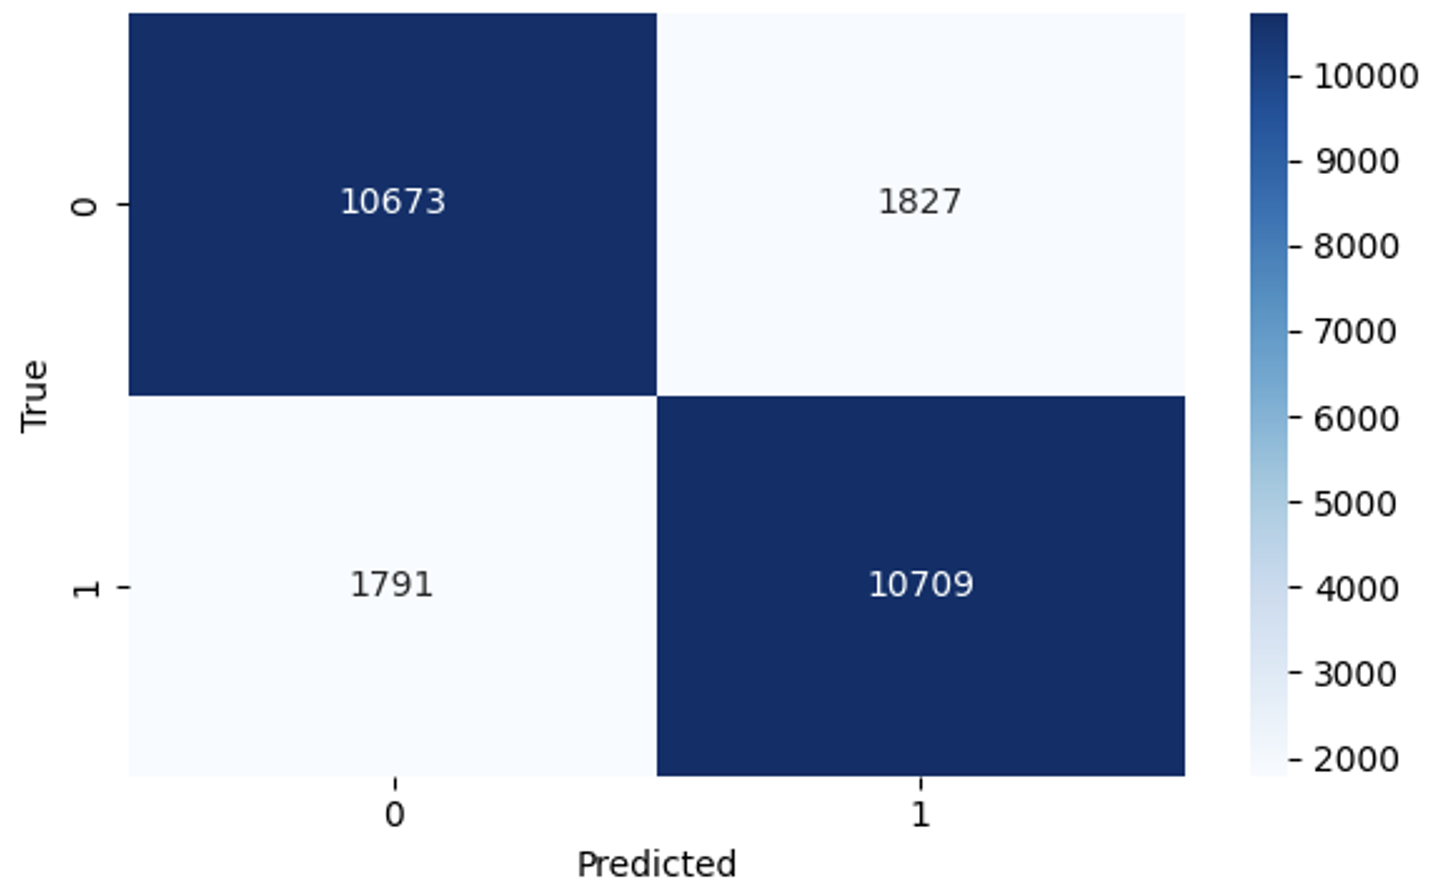
\includegraphics[width=0.5\textwidth]{pics/lstm_metrix.png}
    \caption{The confusion matrix of LSTM}
\end{figure}

\subsection{Optimization on epochs}
In the "Accuracy on epochs" plot, the learning curve of the LSTM model is demonstrated clearly. From the training and validation accuracy curves, it is observed that the validation accuracy stabilizes after the 15th epoch, while the training accuracy continues to rise. This phenomenon suggests a risk of overfitting but can be controlled by regularization and monitoring.

\begin{figure}[ht]
    \centering
    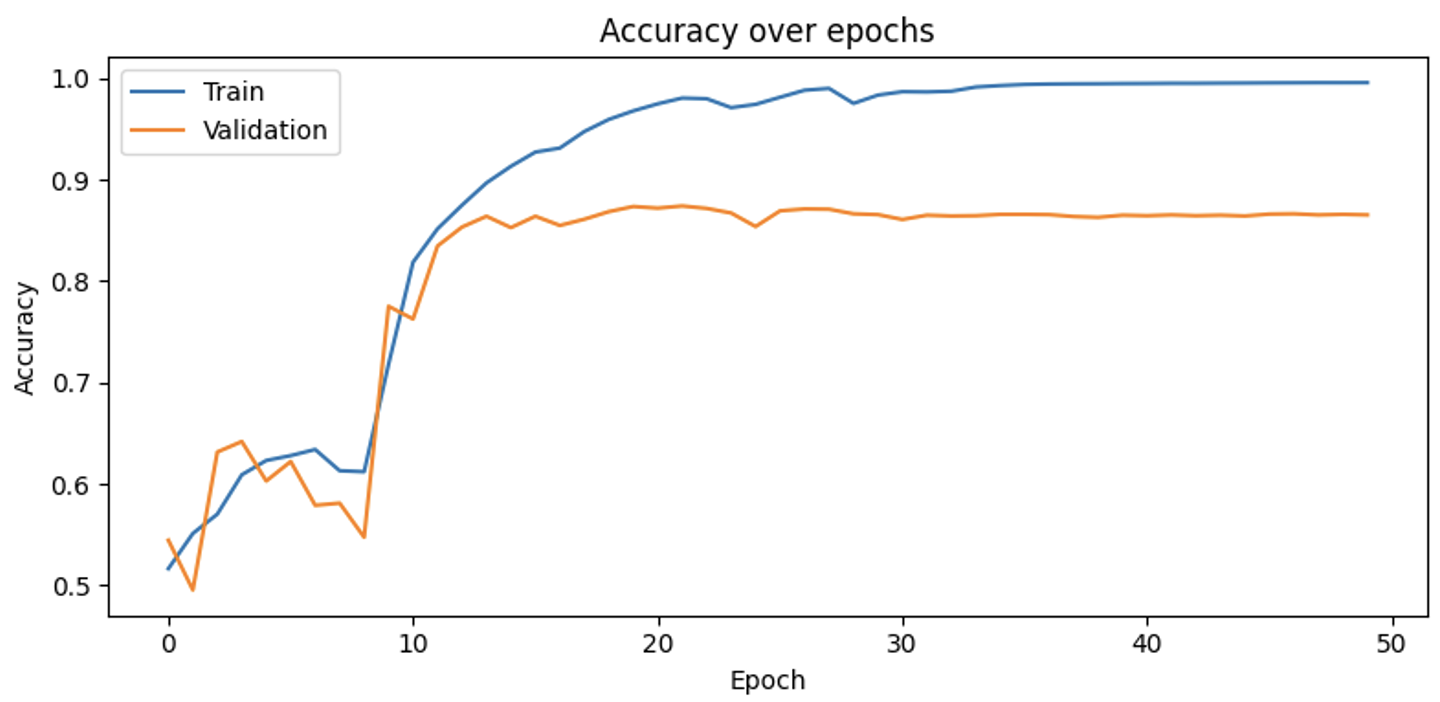
\includegraphics[width=0.5\textwidth]{pics/lstm_accuracy_s.png}
    \caption{Accuracy on epochs of LSTM}
\end{figure}

\subsection{Conclusion}
In summary, LSTM networks offer a powerful and balanced solution for sentiment analysis on the IMDb dataset that outperforms traditional methods and achieves robust and unbiased results. In the future, we can try to make some improvements including the integration of pre-trained word vectors, attention mechanisms, or more sophisticated regularisation techniques, as well as a more formal assessment of the model's statistical significance and generalisation capabilities.






\section{Methodology of BERT}

BERT is a powerful natural language processing (NLP) model developed by Google in 2018. It based on the bidirectional architecture to understand context of words by consider the words before and after them in the sentence. It can be configured to handle multiple type of tasks, the classification task like this sentiment identifying is one of its ability. Hugging Face is an open-source platform and popular for its "Transformers" library, which provides utilities to work with models like BERT. This platform do not maintain the model, but it plays a key role in BERT used widely. Hugging Face hosts pre-trained BERT models and provides code for model using, and established a community for fine tuning and deploying models for verity tasks. BERT and Hugging Face empower developers to tackle a wide range of NLP tasks efficiently.

BERT comes in several variants, each designed for different needs:

\begin{itemize}
    \item BERT-Base: A smaller model with 12 layers, suitable for tasks with limited computational resources like this task.
    \item BERT-Large: A larger model with 24 layers, offering higher accuracy but requiring more computing resource such as GPUs and memory.
    \item DistilBERT: A distilled and lighter version model with fewer parameters, faster and less resource requirements but slightly less accurate.
    \item Multilingual BERT: Trained on textual content from multiple languages, it is useful for non-English or cross-lingual tasks.
\end{itemize}

BERT is the resource and time consuming method due to it based on transformer architecture and attention mechanism. We selected the "BERT-Base" model for this task, it balanced the resources consuming and accuracy of the results. The powerful environment should be used to drive this experiment. We selected the Kaggle platform to handle this task by configuring the system using P100 GPU. It includes CUDA cores and up to 16Gb memory, which support this implementation well.

\begin{figure}[ht]
    \centering
    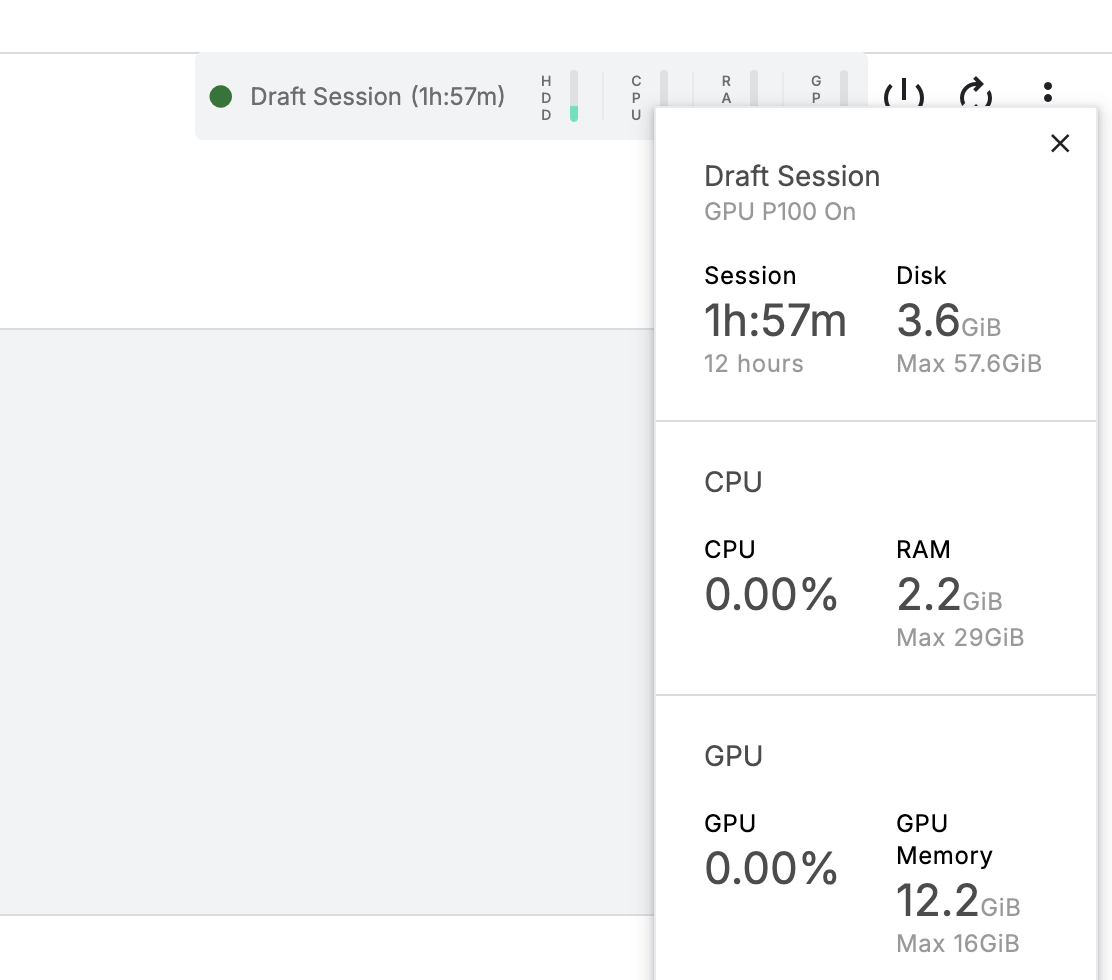
\includegraphics[width=0.4\textwidth]{pics/bert_consuming.png}
    \caption{BERT training environment}
\end{figure}

\subsection{Input data and processing}
This experiment based on BERT and IMDb dataset (like previous experiments). The original "stanfordnlp/imdb" dataset includes training and testing sets, so, we will use the pre-split sets to train and test this time. But we need to tokenize every sample for fine tuning the BERT model configured for classification task.

Compare to the generative LLMs (large language models), BERT needs structured data for its tasks.
The preprocessing steps include tokenizing the textural samples, the "BertTokenizer" from the transforms library, specifically the "google-bert/bert-base-uncased", is used to tokenize the reviews. The preprocessing follows the next steps:

\begin{enumerate}
    \item Tokenization: Converts raw content into tokens compatible with BERT.
    \item Truncation and Padding: Ensures all textual inputs are filled to a maximum length of 512 (in this experiment setting) tokens and padded to maintain uniform input size.
    \item Batched Processing: The training and testing sets are tokenized in batches to improve efficiency.
\end{enumerate}

\begin{figure}[ht]
    \centering
    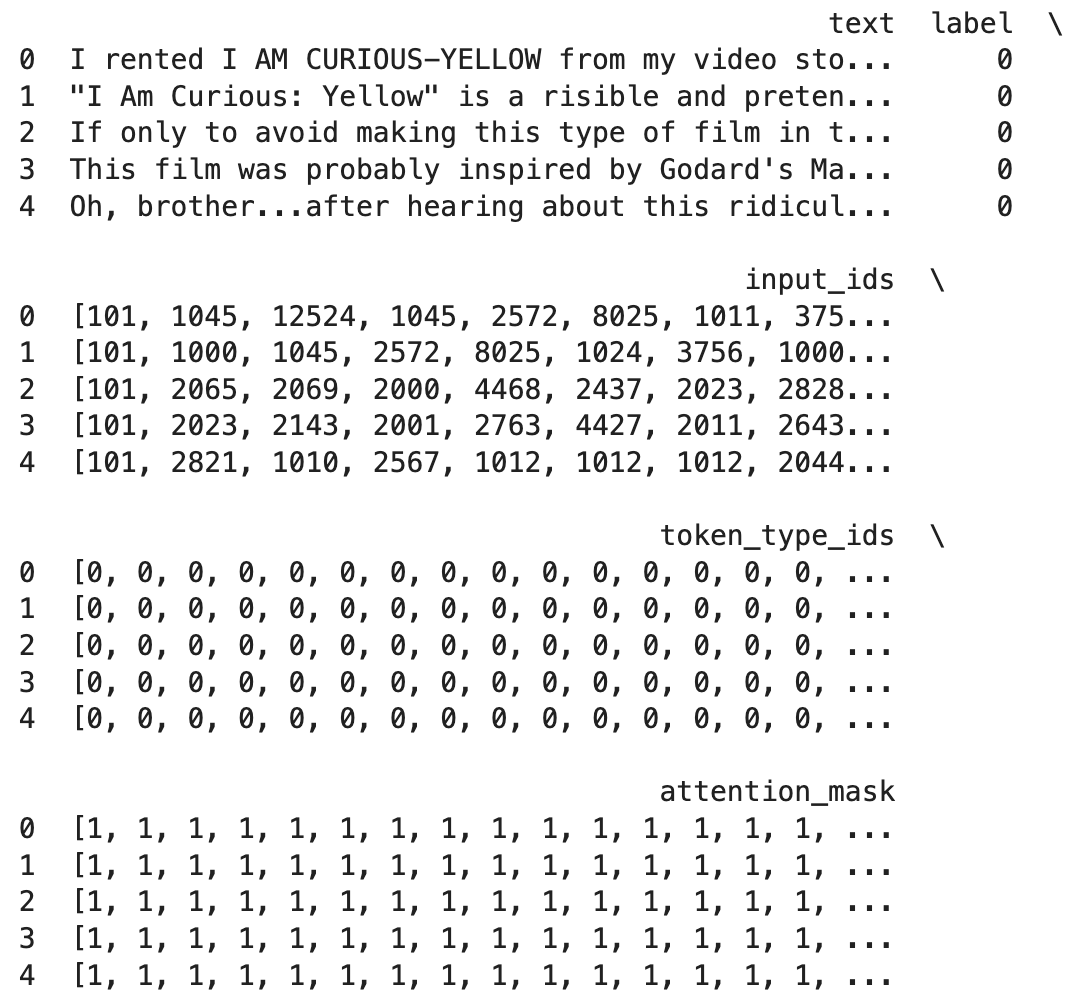
\includegraphics[width=0.6\textwidth]{pics/bert_data_treate.png}
    \caption{The structured data for BERT}
\end{figure}

\subsubsection*{Reasons for Tokenization}

\begin{itemize}
    \item Model Compatibility: BERT models require formatted inputs as the numerical token IDs instead of raw text. This process converts words into the IDs based on the pre-trained vocabulary dictionary.
    \item Fixed Length: BERT expects inputs with fixed length. 
    \item Efficient Processing: The batch processing is critical for efficient training on large datasets like IMDb.
    \item Special Tokens: BERT requires specific tokens (e.g., [CLS], [SEP]) to indicate the start and end of sequences, this step is done by tokenization automatically.
    \item Attention Masking: Tokenization generates attention masks to differentiate meaningful tokens from whole inputs to improve model efficiency by ignoring padded tokens.
\end{itemize}

\subsubsection*{Fields in Tokenized Data}

The "preprocess\_function" generates the dataset with the following fields for each sample:

\textbf{"input\_ids"}: A list of integers for representing the tokenized words of the review, mapped to the BERT vocabulary. Each ID in this list corresponds to a specific token. For example, the word "movie" might be mapped to a specific ID like 3185. This field is the primary input to the BERT model for processing the text.

\textbf{"token\_type\_ids"}: A list of binary integers (0 or 1) indicates the tokens belong to the first sequence (the review text) or a second sequence (e.g., a question in question-answering tasks). For this tasks with single sequence, such as sentiment classification, all values are typically 0. This field is working for compatibility with tasks involving multiple sequences.

\textbf{"attention\_mask"}: A list of binary integers indicates which tokens should be processed by the model (1 for real tokens, 0 for padding tokens). This list ensures the model ignores padding tokens added to reach the fixed length, and improves computational efficiency.

\textbf{"labels"}: The original label, 0 means negative and 1 means positive, is retained for training and evaluation. This field is also used to compute the loss during training.

% training and optimize
\subsection{Training(fine tuning) BERT model}
The used model is "BertForSequenceClassification", which from the transformers library and is initialized with the "google-bert/bert-base-uncased". This model is configured for binary classification by setting 'num\_labels' as 2. Training is conducted using the "Trainer" API from the transformers library with the following configuration:

\begin{itemize}
    \item Output Directory: Setting it as current dictionary for saving model, images or logs.
    \item Evaluation Strategy: Setting it off for improving training performance with limited resource.
    \item Learning Rate: Setting it as '2e-5', it is a standard choice for fine-tuning BERT models.
    \item Batch Sizes: Setting it as 32 for training and 64 for evaluation to lower time consuming.
    \item Epochs: Setting it as 3 to balance model's convergence and computational efficiency.
    \item Weight Decay: Setting it as 0.01 to prevent overfitting.
    \item Logging: Setting it as closed for much better performance.
\end{itemize}

\subsection{Optimization of Fine tuning}
This training experiences around 2 hours, which is much time consuming compared to the previous methods. This time consuming is the optimized results. For this method, the optimize is focusing on to run faster to ensure the experiment can be finished. So, we canceled the in-processing evaluation and logging which causes much slower training. We just use 3 epochs that normally used to train the model to prevent overfitting. In the future optimization, to use the larger BERT model like "" is the choice for better performance. 

\subsection{The Evaluation of BERT}

Although the evaluation strategy was set to "no" during training, after training, we can get "eval\_loss" as 0.2147 by invoking "trainer.evaluate" under training all samples. This value is lowering belong the number of samples increasing. The test dataset "tokenized\_test" is prepared for next post-training evaluation. The model is evaluated by Confusion Matrix, Classification Report and ROC Curve by importing "sklearn.metrics".

\begin{figure}[ht]
    \centering
    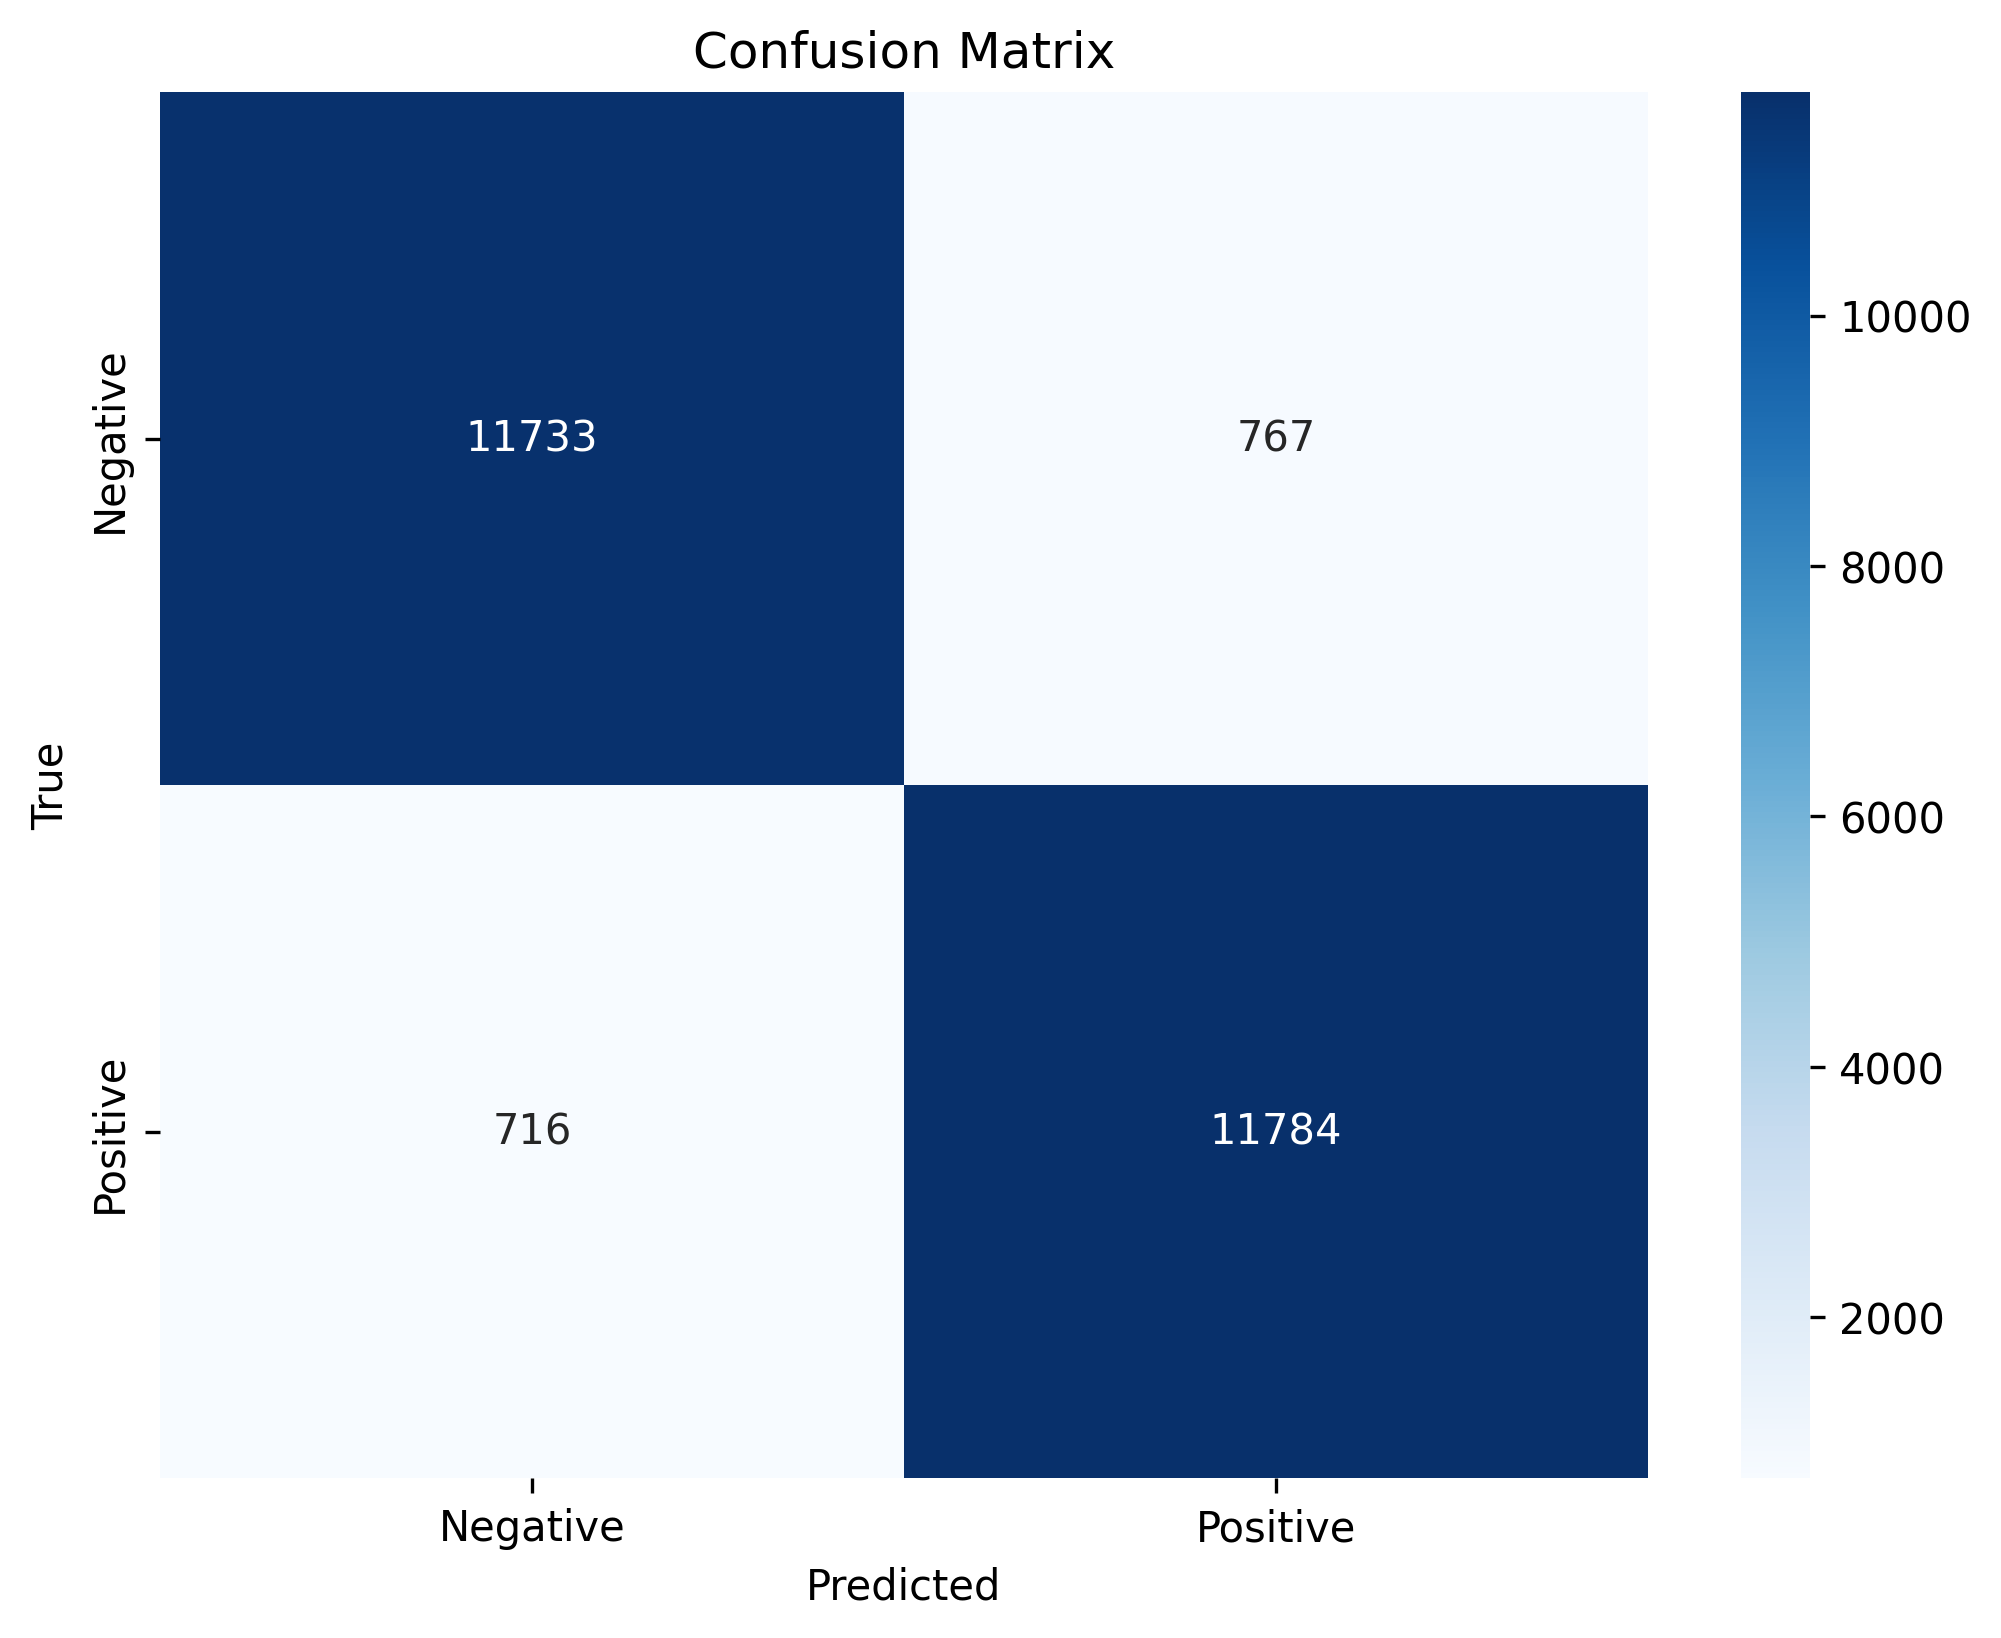
\includegraphics[width=0.4\textwidth]{pics/bert_matrix.png}
    \caption{Confusion Matrix of BERT}
\end{figure}

It is clear that the true positive and true negative is significantly higher than the false negative and false positive, which means that the performance of BERT in this task is much near the 100\%. Depend on the Classification Report of BERT, this experiment also demonstrate the clear trend. The total accuracy is 94\%, and the positive and negative subsets accuracy is also the same values due to the balanced dataset. The precision, f1 score and recall are also reached the perfect range of value.

The Receiver Operating Characteristic (ROC) curve for the BERT model illustrates its better performance in classifying task for positive and negative reviews, the curve demonstrates strong discriminative ability. The curve is expected to close the top-left corner, which reflects high True Positive Rate (TPR), and it gives the low evaluation loss of 0.2147 from "trainer.evaluate" method. 

\begin{figure}[ht]
    \centering
    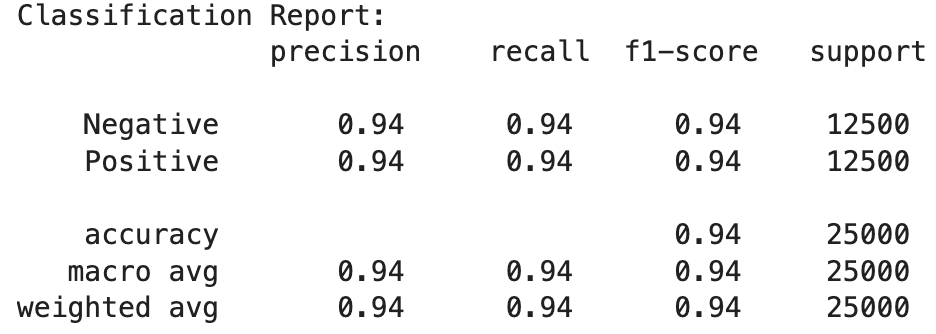
\includegraphics[width=0.5\textwidth]{pics/bert_eval_report.png}
    \caption{Classification Report of BERT}
\end{figure}

\begin{figure}[ht]
    \centering
    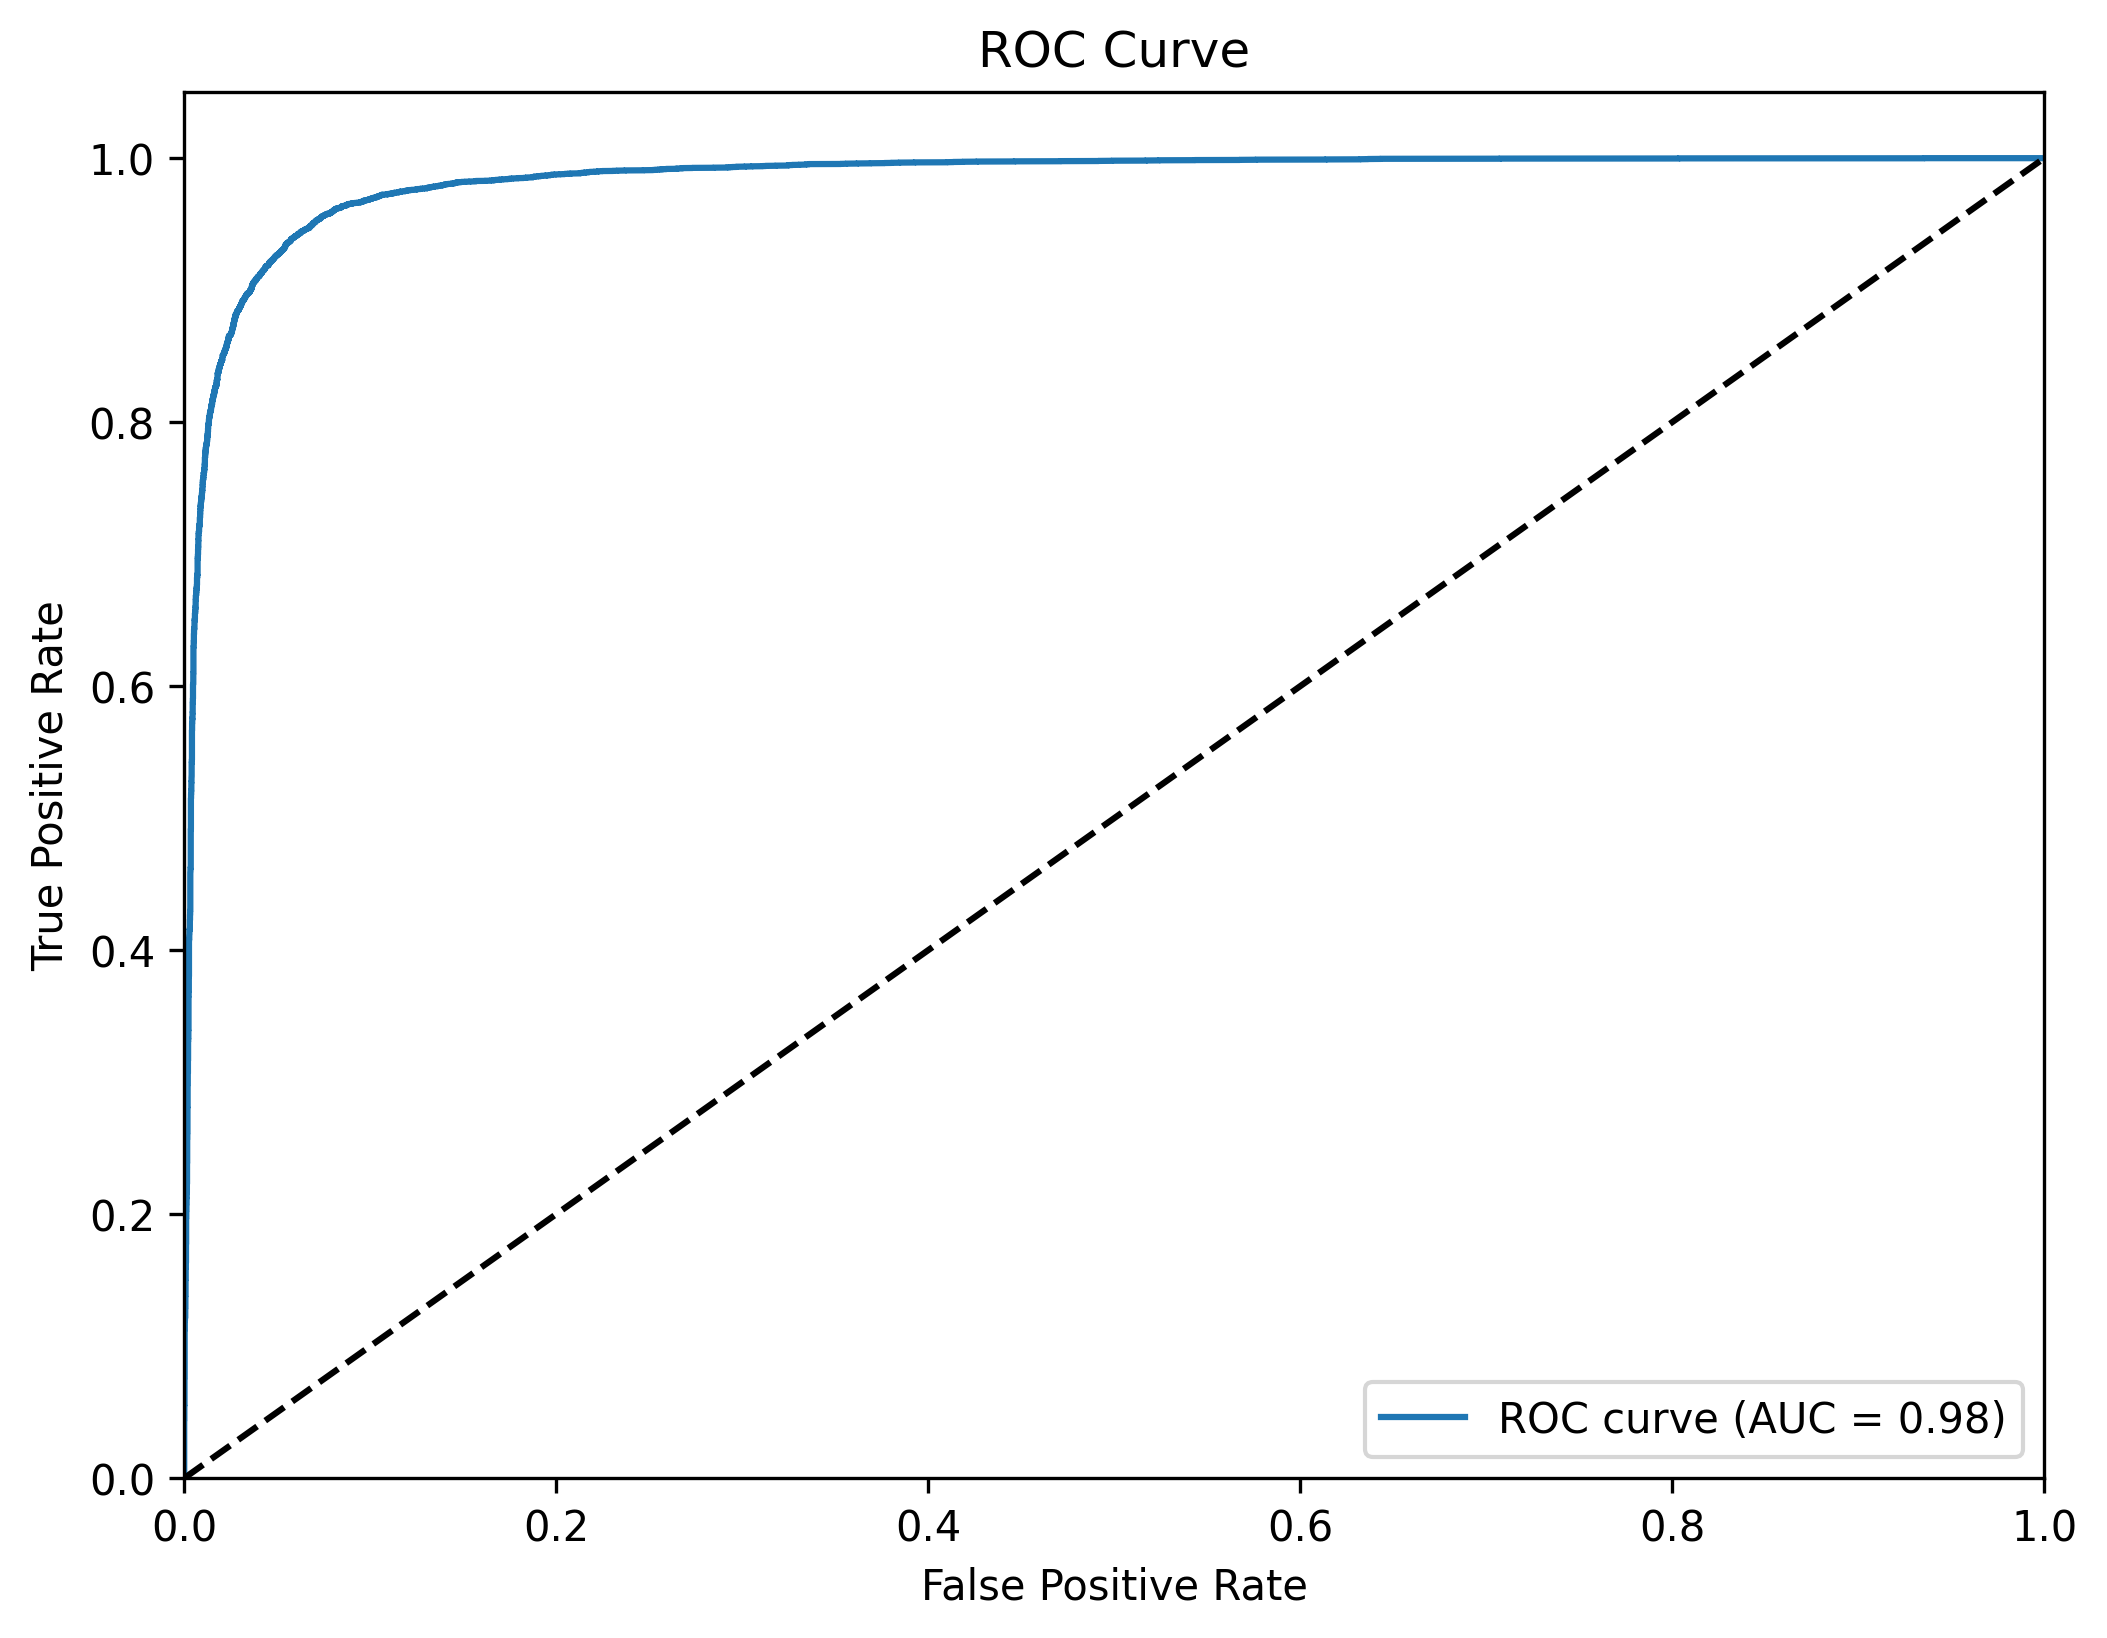
\includegraphics[width=0.5\textwidth]{pics/bert_roc_curve.png}
    \caption{ROC Curve of BERT}
\end{figure}

\subsection{Conclusion}
The experiment of this part demonstrates the successful application of the BERT model for sentiment classification on the IMDb dataset. The steady decrease in training loss over 2,346 steps indicates that the model effectively learned to classify movie reviews by positive or negative. The use of standard preprocessing techniques, such as tokenization with truncation and padding, ensure compatibility with BERT's input requirements. The training configuration, leveraging the Trainer API and GPU acceleration, was efficient and robust.
\section{Final discuss and Recommendation}

\textbf{Random Forest} achieved 85.4\% accurate rate on the IMDb test set. As a traditional machine learning model, it relies on feature engineering (e.g., TF-IDF vectors) and decision tree ensembles. Its strengths include computational efficiency, minimal hardware requirements (trainable on CPUs), and interpretability. However, its accuracy lags means that it unable to capture complex semantic relationships in the sequence, which limits its performance compared to neural network models.

\textbf{LSTM} recorded an accuracy of 85.5\%, it is slightly outperforming Random Forest, reflecting better handling of sequential data. As a recurrent neural network, it excels at modeling the sequential nature of text, which makes it suitable for capturing the flow of sentiments in reviews. It requires moderate computational resources, and less demanding than transformer models, offering a balance between performance and efficiency. However, its accuracy is limited by its unidirectional processing and struggling with long dependencies, this feature lead to lower performance compared to more advanced architectures.

\textbf{BERT} achieved an outstanding 94\% accuracy on the test set, with an evaluation loss of 0.2147, it demonstrates strong generalization. Its ROC curve is expected to approach the top-left corner and an AUC is 0.98, which indicates excellent ability to distinguish positive and negative sentiments. BERT's transformer architecture is pre-trained to handle vast text, and it is fine-tuned on IMDb for capturing bidirectional context and complex linguistic patterns. Its major downside is computational intensity, the experiment requires significant resources depend on the start of BERT methodology. Moreover, its complex architecture reduces interpretability compared to Random Forest.

BERT's 94\% accuracy significantly surpasses Random Forest and LSTM. The result highlights the superiority of transformers in capturing text semantics. For future work, to explore lighter transformers like DistilBERT for efficiency. If resources are limited, the Random Forest with word embeddings or opt for LSTM is suitable. For top performance, BERT remains the best choice.


\clearpage
\bibliographystyle{ieeetr}
\bibliography{ref}

\end{document}

